\documentclass{llncs}

\usepackage{tabularx}
\usepackage{makeidx}  % allows for indexgeneration
\usepackage{amsfonts}
\usepackage{amsmath}
%\usepackage{natbib}
\usepackage{graphicx}
\usepackage{tikz}
\usepackage{mathtools}
\usetikzlibrary{chains,fit,shapes,calc}
\usepackage{verbatim}
\usepackage{semantic}
\usepackage{tabu}
\usepackage{mathptmx}
\usepackage{todonotes}
\newcommand{\concat}{\ensuremath{+\!\!\!\!+\,}}  

%\newtheorem{prop}{Proposition}
%\newtheorem{lemma}{Lemma}
%\newtheorem{defin}{Definition}

\begin{document}

\title{Cactus Environment Machine}
\subtitle{Shared Environment Call-by-Need}

\author{George Stelle\inst{1,2} \and Darko Stefanovic\inst{1} 
        \and Stephen L. Olivier\inst{2} 
        \and Stephanie Forrest\inst{1}
        }
      
\institute{University of New Mexico  \\
\email{\{stelleg, darko, forrest\}@cs.unm.edu}
\and Sandia National Laboratories \\
\email{slolivi@sandia.gov}}

\maketitle
\setcounter{footnote}{0}

\begin{abstract}
Existing machines for lazy evaluation use a \emph{flat} representation of
environments, storing the terms associated with free variables in an array.
Combined with a heap, this structure supports the shared intermediate results
required by lazy evaluation.  We propose and describe an alternative
approach that uses a \emph{shared} environment to minimize the overhead of
delayed computations. We show how a shared environment can act as both an
environment and a mechanism for sharing results. To formalize this approach, we
introduce a calculus that makes the shared environment explicit, as well as
a machine to implement the calculus, the \emph{Cactus Environment Machine}. A
simple compiler implements the machine and is used to run experiments for
assessing performance. The results show reasonable performance and suggest that
incorporating this approach into real-world compilers could yield performance
benefits in some scenarios.
\end{abstract}

\section{Introduction}

Call-by-need evaluation is a formalization of the idea that work
should be delayed until needed, and performed only once.  Existing
implementations of call-by-need take care in \emph{packaging} a delayed
computation, or \emph{thunk}, by building a closure with an array that contains
the bindings of all free variables \cite{jonesstg,boquist1997grin}. The overhead
induced by this operation is well known, and is one reason existing implementations
avoid thunks wherever possible \cite{johnsson1984efficient}. The key insight of
our Cactus Environment ($\mathcal{\mathcal{C} \mskip -4mu \mathcal{E}}$) Machine is that this overhead can be
minimized by only recording a location in a shared environment.

As an example, consider the application $f \; e$. In existing call-by-need
implementations, e.g., the STG machine\cite{jonesstg}, a closure with a flat
environment will be constructed for $e$.  Doing so incurs a time and memory cost
proportional to the number of free variables of $e$. \footnote{In some
implementations, these are lambda-lifted to be formal parameters, but the
principle is the same.} We minimize this packaging cost by recording a
location in a shared environment, which requires only two
machine words (and two instructions) for the thunk: one for the code pointer,
and one for the environment pointer. One way to think about the approach is that
it is \emph{lazier} about lazy evaluation: in the case that $e$ is unneeded, the
work to package it in a thunk is entirely wasted. In the spirit of lazy
evaluation, we attempt to minimize this potentially unnecessary work.  

The main contributions of the paper are:
\begin{itemize}
\item A big-step calculus and small-step abstract machine that formalize the
notion of a shared environment for call-by-need evaluation using an explicitly
shared environment (Section~\ref{sec:calc}).
\item A simple implementation of the abstract machine that compiles to x86
assembly with a preliminary evaluation that shows performance comparable to
existing implementations (Sections~\ref{sec:impl} and~\ref{sec:eval}).
\end{itemize}

Section~\ref{sec:back} reviews relevant background material, and
Section~\ref{sec:env} discusses the current landscape of environment
representations, highlighting the opportunity for combining shared environments
with lazy evaluation.  We then provide some intuition for why this might be
combination might be desirable, and formalize the connection between call-by-need
evaluation and shared environments in a calculus (Section~\ref{sec:calc}).
Section~\ref{sec:mach} uses the calculus to derive a novel abstract machine,
the $\mathcal{\mathcal{C} \mskip -4mu \mathcal{E}}$ machine, explains how
$\mathcal{\mathcal{C} \mskip -4mu \mathcal{E}}$ uses the shared environment in
a natural way to implement lazy evaluation, and gives its formal semantics.  We
then describe a straightforward implementation of $\mathcal{\mathcal{C} \mskip
-4mu \mathcal{E}}$ in Section~\ref{sec:impl}, extended with machine literals
and primitive operations, and compiling directly to native code. We evaluate the
implementation in Section~\ref{sec:eval}, showing that it is capable of
performing comparably to existing implementations despite lacking several
common optimizations, and we discuss the results. We discuss related work, the
limitations of our approach, and some ideas for future work in
Section~\ref{sec:disc}, and conclude the paper in Section~\ref{sec:conc}.



\section{Background and Motivation} \label{sec:back}

This section provides relevant background for the $\mathcal{CE}$ machine,
outlining lambda calculus, evaluation strategies, and Curien's calculus of
closures.

\subsection{Preliminaries}

We begin with the simple lambda calculus:  $$ t::= x \; | \;  \lambda x.t \; |
\;  t \; t $$ where $x$ is a variable, $\lambda x.t$ is an abstraction, and $t
\; t$ is an application. We also use lambda calculus with deBruijn indices,
which replace variables with a natural number indexing into the binding lambdas.
This calculus is given by the syntax: $$ t::= i \; | \; \lambda t \; | \; t \; t
$$ where $i \in \mathbb{N}$. In both cases, we use the standard Barendregt
syntax conventions, namely that applications are left associative and the bodies
of abstractions extend as far as possible to the right
~\cite{barendregt1984lambda}.  A \emph{value} in lambda calculus refers to an
abstraction. We are concerned only with evaluation to weak head normal form
(WHNF), in which evaluation terminates on an abstraction without entering its
body.

In mechanical evaluation of expressions, it would be too inefficient to perform
explicit substitution. To solve this, the standard approach uses closures
~\cite{landin1964mechanical,curien1991abstract,jonesstg,biernacka2007concrete}.
Closures combine a term with an environment, which binds the free variables in
the term to closures. 

For a formal basis, we use Curien's calculus of closures, given in
Figure~\ref{fig:calcclos}~\cite{curien1991abstract}.  It is a formalization of
closures with an environment represented as a list of closures, indexed by
deBruijn indices. We will occasionally modify this calculus by replacing the
deBruijn indices with variables for readability, in which case variables are
looked up in the environment instead of indexed, e.g., $t[x = c, y = c'])$
~\cite{barendregt1984lambda}. We also add superscript and subscript markers to
denote unique syntax elements, e.g., $t', t_1 \in \textnormal{Term}$. 

\subsection{Evaluation Strategies} \label{sec:eval}

There are three evaluation strategies for lambda calculus worth noting:
call-by-value, call-by-need, and call-by-name.  Call-by-value evaluates every argument
to a value, whereas call-by-need and call-by-name only evaluate an argument if
it is needed.  If an argument is needed more than once, call-by-name re-computes
the value, where call-by-need memoizes the value, so it is computed at most once.
Thus, call-by-need attempts to embody the best of both worlds---never repeat
work (call-by-value), and never perform unnecessary work (call-by-name). These
are intuitively \emph{good} properties to have, and we illustrate the
correctness of such an intuition with the following example, modified from
~\cite{danvy2013synthetic}:

$$ \overbrace{c_m (c_m (\cdots(c_m}^{m} \; id \;  id)\cdots) id) \; true \; id
\; bottom $$ where $c_n = \lambda s.\lambda z.\overbrace{s \; (s \cdots (s}^{n}
\; z) \cdots) $, $true = \lambda t.\lambda f.t$, $id=\lambda x.x$, and $bottom =
(\lambda x.x \; x) \lambda x.x \; x$. Call-by-value never terminates,
call-by-name takes exponential time, and call-by-need takes only polynomial time
~\cite{danvy2013synthetic}. Of course, this is a contrived example, but it
illustrates why call-by-need has some desirable properties.

In practice, however there are significant issues with call-by-need evaluation.
We focus on the following issue: \emph{Delaying a computation is slower than
performing it immediately.} This issue is well known in the literature, and has
become part of the motivation for a tool called \emph{strictness analysis},
which transforms non-strict evaluation to strict when possible
\cite{mycroft1982abstract,wadler1987projections}. 

\subsection{Existing Call-by-Need Machines}

Diehl et al. ~\cite{diehl2000abstract} review the call-by-need
literature in detail.  Here we summarizes a few key points.

The best known machine for lazy evaluation is the Spineless Tagless
G-Machine (STG machine), which underlies the Glasgow Haskell Compiler (GHC). 
STG uses flat environments that can be allocated on the stack, the heap,
or some combination ~\cite{jonesstg}. The STG machine is the
most widely used lazy evaluation machine. 

Two other influential lazy evaluation machines relevant to the $\mathcal{CE}$
machine are: the call-by-need Krivine machines
~\cite{lkm,krivine2007call,sestoft}, and the three instruction machine (TIM)
~\cite{TIM}.  Krivine started as an approach to call-by-name evaluation, and was
later extended to call-by-need
~\cite{krivine2007call,sestoft,danvy2013synthetic,lkm}.  The $\mathcal{CE}$
modifies the lazy Krivine machine to capture the environment sharing given by
the cactus environment. The TIM is an influential
implementation of call-by-need and call-by-name ~\cite{TIM}.  It involves, as
the name suggests, three machine instructions, \texttt{TAKE}, \texttt{PUSH}, and
\texttt{ENTER}. In Section~\ref{sec:impl}, we follow Sestoft ~\cite{sestoft} and
re-appropriate these instructions for the $\mathcal{CE}$ machine.

There has also been recent interest in \emph{heapless} abstract
machines for lazy evaluation. Danvy et al. ~\cite{danvy2012inter} and
Garcia et al.  ~\cite{garcia2009lazy}, independently derived similar
machines from the call-by-need lambda calculus
~\cite{ariola1995call}. We will return to this work in
Section~\ref{sec:disc}.  These are interesting approaches, but it is
not yet clear how these machines could be implemented efficiently.

\section{Environment Representations} \label{sec:env}

As mentioned in Section~\ref{sec:back}, environments bind free variables to
closures. There is significant flexibility in how they can be represented. In
this section we review this design space in the context of existing work, both
for call by value and call by need.\footnote{Some work refers to this
space as \emph{closure} representation rather than \emph{environment}
representation~\cite{shao1994space,appel1988optimizing}.  Because the term
part of the closure is simply a code pointer and the
interesting design choices are in the environment, we refer to
the topic as environment representation.}

There are two common approaches that span the design space for environment
representation: \emph{flat} environments and \emph{shared} environments (also
known as linked environments)~\cite{appel1988optimizing,shao1994space}. A flat
environment is one in which each closure has its own record of the terms 
its free variables are bound to. A shared environment is one in which parts of
that record are shared among multiple
closures~\cite{appel1988optimizing,shao1994space}. For example, consider the
following term: $$(\lambda x.(\lambda y.t) (\lambda z.t_1)) t_2$$ Assuming the
term $t$ has both $x$ and $y$ as free
variables, we must evaluate it in the environment binding both $x$ and $y$.
Similarly, assuming $t'$ contains both $z$ and $x$ as free variables, we must
evaluate it in an environment containing bindings for both $x$ and $z$. Thus, we
can represent the closure for evaluating $t$ and $t_1$  as $$t[x=t_2[\bullet],
y=c]$$ and $$t_1[x=t_2[\bullet], z=c_1]$$ respectively.  These are examples of
\emph{flat} environments, where each closure comes with its own record of all of
its free variables. Because of the nested scope of the given term, $x$ is bound
to the same closure in each environment.  Thus, we can also create a shared,
linked environment, represented by the following diagram:

\begin{center}
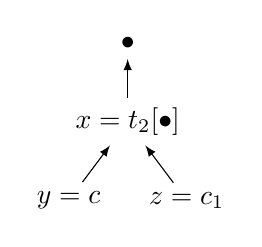
\begin{tikzpicture}[ 
  edge from parent path={(\tikzchildnode\tikzchildanchor) edge [-latex] (\tikzparentnode\tikzparentanchor)},
  level distance=1cm
]
\node (d) {$\bullet$} child{node (a) {$x=t_2[\bullet]$} child{node (b) {$y=c$}} child{node (c)
{$z=c_1$}}};

\end{tikzpicture}
\end{center}
Now each of the environments is represented by a linked list, with the binding
of $x$ shared between them. This is an example of a \emph{shared} environment
~\cite{appel1988optimizing}. This shared, linked structure dates back to the 
first machine for evaluating expressions: Landin's SECD
machine~\cite{landin1964mechanical}.

The drawbacks and advantages of each approach are well known. With a flat
environment, variable lookup can be performed with a simple offset
~\cite{jonesstg,appel2006compiling}. On the other hand, significant
duplication can occur, as we will discuss in Section~\ref{sec:exist}.
With a shared environment, that duplication is removed, but at the cost of
possible link traversal upon dereference. 

As with most topics in compilers and abstract machines, the design space is
actually more complex. For example, Appel and Jim show a wide range of hybrids
~\cite{appel1988optimizing} between the two, and Appel and Shao
~\cite{shao1994space} show an optimized hybrid that aims to achieve the benefits
of both approaches. And as shown in the next section, choice of evaluation
strategy further complicates the picture.

\subsection{Existing Call-by-Need Environments} \label{sec:exist}

Existing call by need machines use flat environments with a heap of
closures~\cite{jonesstg,TIM,johnsson1984efficient,boquist1997grin}. These
environments may hold some combination of primitive values and pointers into the
heap. The pointers and heap implement the memoization of results required for
call by need. Returning to the earlier example, $(\lambda x.(\lambda y.t)
(\lambda z.t_1)) t_2$, we can visualize the execution state when entering $t$ as
follows:

\begin{center}
\textbf{Closure}
\begin{align*}
t[x=p, y=p_1] \\
\end{align*}
\textbf{Heap}
\begin{align*}
p &\mapsto t_2[\bullet] \\
p_1 &\mapsto \lambda z.t_1[x=p] 
\end{align*}
\end{center}

If $t_2[\bullet]$ is not in WHNF (this sort of unevaluated closure is called a
\emph{thunk}~\cite{ingerman1961way,peyton1992implementing}), then if it is
entered in either the evaluation of $t$ or $t_1$, the resulting value will
overwrite the closure at $p$. The result of the computation is then shared with
all other instances of $x$ in $t$ and $t_1$. 

To better understand one of the costs of flat environments, consider the
following example: $$\lambda g.\lambda x.\lambda y.\lambda z.g
\; t \;t'$$ Without any preprocessing, the standard cost of duplication applies:
if $x$, $y$, and $z$ are free in $t$ and $t'$, then $t$ and $t'$ will have
large, identical environments and their closures will be expensive to create.
Compile-time transformation ~\cite{peyton1992implementing} (tupling arguments)
helps, but it is not clear that the technique extends to the general case. We
claim that the machine itself should avoid duplicating environments.

Depending on $g$, either or both of the closures created for its arguments may
not be evaluated.  Therefore, it is possible that the work of creating the
environment for that thunk will be wasted. This waste is well known, and
existing approaches address it by avoiding thunks as much as possible
~\cite{jonesstg,johnsson1984efficient}. Unfortunately, in cases like the above
example, this is impossible; the thunks are necessary. Indeed, even if we tuple
the closures for $x$, $y$, and $z$, that tuple could be wasted if neither $t$ nor
$t'$ is used. Thus, we would like to minimize the cost of creating such thunks.

Thunks are special in another way.  Recall the standard advantage of the flat
environment: quick variable lookups. In a lazy language, this advantage is
lessened by the following fact: \emph{a thunk can only be entered once}. After
it is entered, it will be overwritten with a value, so the next time that heap
location is entered it will be entered with a value and a different environment.
Thus, the work to ensure that the variable lookup is fast will be used only
once. This is in contrast to a call by value language, in which every closure is
constructed for a value, which can be entered an arbitrary number of times. 

A more subtle drawback of the flat environment representation is that
environments can vary in size, and thus a value in WHNF can be too large to fit
in the space allocated for the thunk it is replacing. This problem is discussed
in~\cite{jonesstg}, where the proposed solution is to put the value closure in
a fresh location in the heap where there is sufficient room. The original
thunk location is then replaced with an indirection to the value at the freshly
allocated location. These indirections are removed during garbage collection,
but do impose some cost, both in runtime efficiency and implementation
complexity~\cite{jonesstg}.

We have thus far ignored a number of details with regard to current
implementations. For example, the STG machine can split the flat environment, so
that part is allocated on the stack and part on the heap.  The TIM allocates its
flat environments separately from its closures so that each closure is a code
pointer, environment pointer pair~\cite{TIM}. while the STG machine keeps
environment and code co-located~\cite{jonesstg}. Still, the basic design
principle holds: a flat environment for each closure allows quick variable
indexing, but at the costs given above.

An intuitive view of the flat environment representation in a call by need
language is that whenever a term might be needed, the necessary environment is
constructed from the current environment.  This operation is expensive, and
it is wasted if the variable is never entered. This potentially wasted cost is
one of the primary motivations for the current work: \emph{lightweight
closure creation}. In other words, we would like to minimize the cost of saving
the current environment.

See Figure~\ref{fig:designspace} for a simple summary of the design space
relevant to this paper. There are existing call by value machines with both flat
and shared environments, and call by need machines with flat environments. As
far as we are aware, we are the first to use a shared environment to implement
lazy evaluation.

\begin{figure}
\begin{tabularx}{\textwidth}{l | X | X}
                & Flat Environment     & Shared Environment \\ \hline
  Call by need  & STG, TIM, GRIN & $\mathcal{CE}$ Machine (this paper) \\
  Call by value & ZAM, SML & ZAM, SECD, SML \\
\end{tabularx}
\caption{Evaluation strategy and environment structure design space. Each
acronym refers to an existing implementation. Some implementations use multiple
environment representations.}
\label{fig:designspace}
\end{figure}


\section{Cactus Environment Calculus} \label{sec:calc}

This section shows how the shared environment approach can be applied to
call-by-need evaluation. We start with a calculus that abstracts away
environment representation, Curien's calculus of closures, and we show how it
can be modified to force sharing. See Curien's call-by-name calculus of closures
in Figure~\ref{fig:calcclos}. \footnote{Curien calls it a ``lazy'' evaluator, and
there is some ambiguity with the term lazy, but we use the term only to mean
call-by-need. We also remove the condition checking that $i < m$ because we are
only concerned with evaluation of closed terms.}

The LEval rule pushes a closure onto the environment, and the LVar rule indexes
into the environment, entering the corresponding closure. We show in this
section that by removing ambiguity about how the environments are represented,
and forcing them to be represented in a \emph{cactus stack}
~\cite{stenstrom1988vlsi}, we can define our novel call-by-need calculus.

\begin{figure}
\textbf{Syntax}
\begin{align*}
\tag{Term} t &::= i \; | \; \lambda t \; | \; t \; t  \\
\tag{Variable} i &\in \mathbb{N}  \\
\tag{Closure} c &::= t [\rho] \\
\tag{Environment} \rho &::= \bullet \; | \; c \cdot \rho \\
\end{align*}
\textbf{Semantics}
\begin{align*}
\tag{LEval}\inference
{t_1[\rho] {\xrightarrow{* }}_L \lambda t_2[\rho'] }
{t_1 t_3[\rho] \rightarrow_L t_2[t_3[\rho] \cdot \rho'] } 
\end{align*}
\begin{align*}
\tag{LVar} i [c_0 \cdot c_1 \cdot ... c_i \cdot \rho] \rightarrow_L c_i
\end{align*}
\caption{Curien's call-by-name calculus of closures ~\cite{curien1991abstract}}
\label{fig:calcclos}
\end{figure}

To start, consider again the example from Section~\ref{sec:env}, this
time with deBruijn indices: $(\lambda(\lambda t) \; (\lambda t_1)) t_2$.  The
terms $t$ and $t_1$, when evaluated in the closure calculus, would have the
following environments, respectively: 

\begin{center}
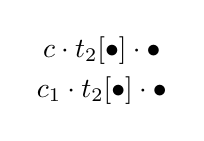
\begin{tikzpicture}
\node {$c \cdot t_2[\bullet] \cdot \bullet$};
\node [yshift=-0.5cm] {$c_1 \cdot t_2[\bullet] \cdot \bullet$};
\end{tikzpicture}
\end{center}

Again, the second closure is identical in each environment.  And again,
we can represent these environments with a shared environment, this time
keeping call-by-need evaluation in mind:
\begin{center}
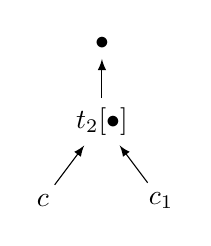
\begin{tikzpicture}[ 
  edge from parent path={(\tikzchildnode\tikzchildanchor) edge [-latex] (\tikzparentnode\tikzparentanchor)},
  level distance=1cm
]
\node (a) {$\bullet$} child{node (d) {$t_2[\bullet]$} child{node (b) {$c$}} child{node (c)
{$c_1$}}};

%\draw let \p1=(a), \p2 =(b), \n1={atan2(\y2-\y1,\x2-\x1)}, \n2={veclen(\y2-\y1,\x2-\x1)}
%  in ($ (a)!0.5!(b) $) ellipse [x radius=\n2/2+10pt, y radius=10pt, rotate=90-\n1];
%\draw let \p1=(a), \p2 =(c), \n1={atan2(\y2-\y1,\x2-\x1)}, \n2={veclen(\y2-\y1,\x2-\x1)}
%  in ($ (a)!0.5!(c) $) ellipse [x radius=\n2/2+10pt, y radius=10pt, rotate=90-\n1];
\end{tikzpicture}
\end{center}
This inverted tree structure seen earlier with the leaves pointing toward the
root is called a \emph{cactus stack} (sometimes called a spaghetti stack or
saguaro stack) \cite{hauck1968burroughs,ichbiah1991rationale}. In this
particular cactus stack, every node defines an environment as the sequence of
closures in the path to the root.  If $t_2[\bullet]$ is a thunk, and is updated
in place with the value after its first reference, then both environments would
contain the resulting value. This is exactly the kind of sharing that is
required by call-by-need, and thus we can use this structure to build a
call-by-need evaluator. This is the essence of the cactus environment calculus
and the cactus environment ($\mathcal{CE}$) machine. 

Curien's calculus of closures does not differentiate between flat and shared
environment representations, and indeed, no calculus that we are aware of has
had the need to. Therefore, we must derive a calculus of closures, forcing the
environment to be shared. Because we can hold the closure directly in the
environment, we choose to replace the standard heap of closures with a
\emph{heap of environments}. To enforce sharing, we extend Curien's
calculus of closures to explicity include the heap of environments, which we
refer to as a \emph{cactus environment}. 

See Figure~\ref{fig:calccact} for the syntax and semantics of the cactus
calculus. Recall that we are only concerned with evaluation of closed terms. The
initial closed term $t$ is placed in a $(t[0],\epsilon[0 \mapsto \bullet])$ tuple, and
evaluation terminates on a value. We use the shorthand $\mu(l,i)=l' \mapsto l''
c \dot e$ to say that looking up the $i$'th element in the linked environment
structure starting at $l$ results in location $l'$, where closure $c$ and
continuing environment $e$ reside. We define two different semantics, one for
call-by-name and one for call-by-need, which makes the connection to
Curien's call-by-name calculus more straightfoward. The rule for application
(MEval and NEval) is identical for both semantics: each evaluates the left hand
side to a function, then binds the variable in the cactus environment, extending
the current environment.

The only difference between this semantics and Curien's is that if we need
to extend an environment multiple times, the semantics \emph{requires}
sharing it among the extensions. This makes no real difference for call-by-name,
but it is needed for the sharing of results in the NVar rule. The explicit
environment sharing ensures that the closure that is overwritten with a value is
shared correctly.

\begin{figure*}
\textbf{Syntax}
\begin{align*}
\tag{Term} t &::= i \; | \; \lambda t \; | \; t \; t  \\
\tag{Variable} i &\in \mathbb{N}  \\
\tag{Closure} c &::= t [l] \\
\tag{Value} v &::= \lambda t [l] \\
\tag{Heap} \mu &::= \epsilon \; | \; \mu [ l \mapsto \rho ] \\
\tag{Environment} \rho &::= \bullet \; | \; c \cdot l \\
\tag{Location} l,f &\in \mathbb{N}  \\
\tag{State} s &::= (c, \mu)
\end{align*}
\textbf{Call-by-Name Semantics}
\begin{align*}
\tag{MEval} \inference
{(t[l], \mu) \xrightarrow{* }_{M} (\lambda t_2[l'], \mu') \quad f \not \in \textnormal{dom}(\mu')}
{(t \; t_3[l], \mu) \rightarrow_{M} (t_2[f], \mu'[f \mapsto t_3[l] \cdot l'])}  
\end{align*}
\begin{align*}
\tag{MVar} \inference 
{\mu(l, i) = l' \mapsto c \cdot l''}
{(i[l],\mu) \rightarrow_M (c,\mu)}
\end{align*}
\textbf{Call-by-Need Semantics}
\begin{align*}
\tag{NEval} \inference
{(t[l], \mu) \xrightarrow{* }_{N} (\lambda t_2[l'], \mu') \quad f \not \in \textnormal{dom}(\mu')}
{(t \; t_3[l], \mu) \rightarrow_{N} (t_2[f], \mu'[f \mapsto t_3[l] \cdot l'])}  
\end{align*}
\begin{align*}
\tag{NVar} \inference
{\mu(l, i) = l' \mapsto c \cdot l'' \quad (c, \mu) \xrightarrow{* }_{N} (v, \mu')}
{(i[l],\mu) \rightarrow_N (v, \mu'[l' \mapsto v \cdot l''])}
\end{align*}
\caption{Cactus calculus syntax and semantics.}
\label{fig:calccact}
\end{figure*}

\subsection{Correctness}

Ariola et al. define the standard call-by-need semantics in
~\cite{ariola1995call}. To show correctness, we show that there is a strong
bisimulation between $\rightarrow_{N}$ and their operational
semantics, $\Downarrow$ (Figure~\ref{fig:cbn}). 

\begin{figure}
\begin{align*}
\tag{Id} \inference
{\langle \Phi \rangle t \Downarrow \langle \Psi \rangle \lambda x.t'}
{\langle \Phi, x \mapsto t, \Upsilon \rangle x \Downarrow \langle \Psi, x
\mapsto \lambda x.t', \Upsilon \rangle \lambda x.t'}
\end{align*}
\begin{align*}
\tag{Abs} \inference 
{}
{\langle \Phi \rangle \lambda x . t \Downarrow \langle \Phi \rangle \lambda x.t}
\end{align*}
\begin{align*}
\tag{App} \inference
{\langle \Phi \rangle t_l \Downarrow \langle \Psi \rangle \lambda 
x.t_n \\ \langle \Psi, x' \mapsto t_m \rangle [x'/x]t_n \Downarrow \langle
\Upsilon \rangle \lambda y.t'}
{\langle \Phi \rangle t_l \; t_m \Downarrow \langle \Upsilon \rangle \lambda y.t'}
\end{align*}
\caption{Ariola et. al's Operational Semantics}
\label{fig:cbn}
\end{figure}

{\theorem \textnormal{(Strong Bisimulation)} $$\xrightarrow{}_{N} \; \sim \;
\Downarrow$$}
We start with a \emph{flattening} relation between a configuration for
$\Downarrow$ and a configuration for $\xrightarrow{}_{N}$. The deBruijn indexed
terms and the standard terms are both converted to terms that use deBruijn
indices for local variables and direct heap locations for free variables. The
flattening relation holds only when both terms are closed under their
corresponding heaps. It holds trivially for the special case of initializing
each configuration with a standard term and its corresponding deBruijn-indexed
term, respectively. The proof is finished by induction on the step relation for
each direction of the bisimulation.

\subsection{Recursion}

Correct sharing for recursive data values, as pointed out in
\cite{ariola1995call}, is not possible without adding explicit recursion. We
return to this issue in Section~\ref{sec:disc}, but note here that adding
explicit recursion to this scheme is left for future work.

\section{$\mathcal{CE}$ Machine} \label{sec:mach}

Using the calculus of cactus environment defined in the previous section, we
derive an abstract machine: the $\mathcal{CE}$ machine\footnote{No relation to
Felleisen and Friedman's CEK machine~\cite{felleisen1986control}}. The syntax
and semantics are defined in Figure~\ref{fig:CEM}. 

\begin{figure*}
\textbf{Syntax}
\begin{align*}
\tag{State} s &::= \langle c, \sigma, \mu, f \rangle \\
\tag{Term} t &::= i \; | \; \lambda t \; | \; t \; t  \\
\tag{Variable} i &\in \mathbb{N}  \\
\tag{Closure} c &::= t [l] \\
\tag{Value} v &::= \lambda t[l] \\
\tag{Heap} \mu &::= \epsilon \; | \; \mu [ l \mapsto \rho ] \\
\tag{Environment} \rho &::= \bullet \; | \; c \cdot l \\
\tag{Context} \sigma &::= \square \; | \; \sigma \; c \;  | \; u:=\sigma \\
\tag{Location} l,u,f &\in \mathbb{N}
\end{align*}
\textbf{Semantics}
\begin{align*}
\tag{Upd}
\langle v, u := \sigma, \mu[u \mapsto c \cdot l], f \rangle 
  &\rightarrow_{\mathcal{CE}}
\langle v, \sigma, \mu[u \mapsto v \cdot l], f \rangle  \\
\tag{Lam}
\langle \lambda t[l], \sigma \; c, \mu, f \rangle 
  &\rightarrow_{\mathcal{CE}}
\langle t[f], \sigma, \mu[f \mapsto c \cdot l], f+1 \rangle  \\
\tag{App}
\langle t \; t'[l], \sigma, \mu, f \rangle
  &\rightarrow_{\mathcal{CE}}
\langle t[l], \sigma \; t'[l], \mu, f \rangle \\
\tag{Var1}
\langle 0[l], \sigma, \mu, f \rangle
  &\rightarrow_{\mathcal{CE}}
\langle c, l := \sigma, \mu, f \rangle 
\; \textnormal{where} \; c \cdot l' = \mu(l)\\
\tag{Var2}
\langle i[l], \sigma, \mu, f \rangle
  &\rightarrow_{\mathcal{CE}}
\langle (i-1)[l'], \sigma, \mu, f \rangle
\; \textnormal{where} \; c \cdot l' = \mu(l)
\end{align*}
\caption{Syntax and semantics of the $\mathcal{CE}$ machine.}
\label{fig:CEM}
\end{figure*}

The machine operates on a similar syntax as the calculus, extended only with a
context to implement the updates from the NVar subderivation ($u:=\sigma$) and
the operands from the NEval subderivation ($\sigma \; c$). We also add $f$
explicitly, which is our fresh heap location. Thus, we now have a 4-tuple, with
initial state $\langle t[0], \square, \epsilon[0=\bullet], 1\rangle$. The four
parts of the tuple are the current closure, the context, the heap, and the fresh
heap location. On the update rule, our current closure is a value, and there is
an update marker as the outermost context. This implies that a variable was
entered, and our current closure represents the corresponding value for that
variable.  Thus, we update the location $u$ that the variable entered, replacing
whatever term was entered with the current closure. The Lam rule takes an
argument off the context and binds it to a variable, allocating a fresh heap
location for the bound variable. This ensures that every instance of the
variable will point to this location, and thus the bound term will only be
evaluated at most once. The App rule simply pushes an argument term in the
current environment. The Var1 rule enters the closure pointed to by the
environment location, while the Var2 rule traverses the cactus environment to
locate the correct closure.  

To get some intuition for the $\mathcal{CE}$ machine and how it works, consider
the depiction in Figure~\ref{fig:state} of its state during evaluation of the
term: $(\lambda a.(\lambda b.b \; a) (\lambda c.c \; a)) ((\lambda i.i) (\lambda
j.j))$. We leave the variable names for readability. For thoroughness, the
occurrences of variable $a$ may be replaced with index $1$, and the rest can be
replaced with index $0$. At this point in the computation, the closure for $a$
is shared, and has been updated with its value. The closure in the context (the
$a$ from the application $c \; a$) now points to the updated value.

\begin{figure}
\includegraphics[width=\linewidth]{figures/18.pdf}
The dotted lines represent the environment for the bound closure, and the solid
lines represent the next environment cell:  $t[dotted] \cdot solid$. The
variables are left in for readability, but can be trivially replaced with
deBruijn indices. See Figure~\ref{fig:states} in the Appendix for a
visualization of a number of subsequent machine states. The free Heap location
$f$ is left out to save space.
\caption{$\mathcal{CE}$ machine state example}
\label{fig:state}
\end{figure}

\subsection{Correctness}
We prove that the reflexive transitive closure of the $\mathcal{CE}$ machine
step relation evaluates to a value and heap and empty context iff
$\xrightarrow{}_{M}$ evaluates to the same value and heap.

{\prop \textnormal{(Correctness)} $$(c, \mu) \rightarrow_{M} (v, \mu') \;
\leftrightarrow \; \langle c, \square, \mu \rangle \xrightarrow{*
}_{\mathcal{CE}} \langle v, \square, \mu' \rangle $$} 
By induction on step relations. 

\section{Implementation} \label{sec:impl}

This section describes how the $\mathcal{\mathcal{C} \mskip -4mu \mathcal{E}}$
machine can be mapped directly to x64 insructions. Specifically, we re-define
the three instructions given by the TIM~\cite{TIM}: \texttt{TAKE},
\texttt{ENTER}, and \texttt{PUSH}, and implement them with x64 assembly. We
also describe several design decisions, as well as some optimizations. All
implementation and benchmark code is available at
\texttt{http://cs.unm.edu/\textasciitilde stelleg/cem-tfp2016.tar.gz}.

Each closure is represented as a <code pointer, environment pointer> tuple. The
Context is implemented as a stack, with updates represented as a <null pointer,
environment pointer> tuple to differentiate them from closure arguments. The
Heap, or cactus environment, is implemented as a heap containing <closure,
environment pointer> structs. As a result, each cell in the heap takes 3
machine words.

\subsection{Compilation}
The three instructions are given below, with descriptions of their behavior. 

\begin{itemize}
\item \texttt{TAKE}: Pops a context item off the stack. If the item is an
update $u$, the instruction updates the location $u$ with the current closure.
If it is an argument $c$, the instruction binds the closure $c$ to the fresh
location in the cactus environment.
\item \texttt{ENTER i}: Enters the closure defined by variable index \texttt{i},
the current environment pointer, and the current cactus environment.  \item
\texttt{PUSH m}: Pushes the code location \texttt{m} along with the
current environment pointer. 
\end{itemize}

Each of these instructions corresponds directly to a corresponding lambda term:
abstraction compiles to \texttt{TAKE}, application to \texttt{PUSH}, and
variables to \texttt{ENTER}. Each is compiled using a direct implementation of
the transition functions of the $\mathcal{\mathcal{C} \mskip -4mu \mathcal{E}}$
machine. The mapping from lambda terms can be seen in
Figure~\ref{fig:cemcompile}, which defines the compiler. Unlike the TIM, our
version of \texttt{TAKE} doesn't have an arity; we compile a sequence of
lambdas as a sequence of \texttt{TAKE} instructions.  While we have not
compared performance of the two approaches directly, we suspect that \texttt{n}
inlined \texttt{TAKE} instructions should be roughly as fast as a \texttt{TAKE
n} instruction.  Similarly, the \texttt{ENTER i} instruction can be implemented
either as a loop or unrolled, depending on \texttt{i}, and more performance
comparisons are needed to determine the trade-off between code size and speed.

\begin{figure}
\begin{align*} C[\![t \; t']\!] &= \texttt{PUSH}\;label_{C[\![t']\!]}:C[\![t]\!] \concat C[\![t']\!] \\
C[\![\lambda t]\!] &= \texttt{TAKE}:C[\![t]\!] \\
C[\![i]\!] &= \texttt{ENTER} \; i
\end{align*}
\caption{$\mathcal{\mathcal{C} \mskip -4mu \mathcal{E}}$ machine compilation scheme. $C$ compiles a sequence of
instructions from a term. The $label$ represents a code label: each instruction
is given a unique label. The $:$ operator denotes prepending an item to a
sequence and $\concat$ denotes concatenating two sequences.}
\label{fig:cemcompile}
\end{figure}

We compile to x64 assembly. Each of the three instructions is mapped onto
x64 instructions with a macro. The \texttt{PUSH} instruction is particularly
simple, consisting of only two x64 instructions (two \texttt{push}es, one for
the code pointer and one for the environment pointer). This is actually an
important point: \emph{thunk creation is only two hardware instructions,
regardless of environment size}.  

\subsection{Machine Literals and Primitive Operations}

Following Sestoft~\cite{sestoft}, we extend the $\mathcal{\mathcal{C} \mskip -4mu \mathcal{E}}$ machine to
include machine literals and primitive operations. Figure~\ref{fig:extsyntax}
shows the parts of syntax and semantics that are new or modified. 

\begin{figure}
\textbf{Syntax}
\begin{align*}
\tag{Term}    t &::= i \; | \; \lambda t \; | \; t \; t | \; n \; | \; op \\
\tag{Integer} n &\in \mathbb{I} \\
\tag{PrimOp} op &::= + \; | \; - \; | \; * \; | \; \; / \;\; | \; = \; | \; > \; | \; < \\
\tag{Value} v &::= \lambda t[l] \; | \; n[l] \\
\end{align*}
\textbf{Integer and Primop Semantics}
\begin{align*}
\tag{Int}
\langle n[l], \sigma \; c, \mu, k \rangle
  &\rightarrow_{\mathcal{\mathcal{C} \mskip -4mu \mathcal{E}}}
\langle c, \sigma \; n[l], \mu, k \rangle \\
\tag{Op} 
\langle op[l], \sigma \; n' \; n, \mu, k \rangle
  &\rightarrow_{\mathcal{\mathcal{C} \mskip -4mu \mathcal{E}}}
\langle op(n',n)[l], \sigma, \mu, k \rangle
\end{align*}
\caption{Extensions to the syntax and semantics of the $\mathcal{\mathcal{C} \mskip -4mu \mathcal{E}}$ machine.}
\label{fig:extsyntax}
\end{figure}

\subsection{Omitted Extensions}

Our implementation omits a few other standard extensions. Here we address some
of these omissions.

Data types are a common extension that we omit ~\cite{jonesstg,boquist1997grin}.
We take the approach of Sestoft ~\cite{sestoft} that these can be efficiently
implemented with pure lambda terms. For example, consider a list data type (in
Haskell syntax): \texttt{data List a = Cons a (List a) | Nil}. This can be
represented in pure lambda terms with $Cons = \lambda h.\lambda t.\lambda
c.\lambda n.c \; h \; t$ and $Nil = \lambda c.\lambda n.n$. 

Let bindings are another term commonly included in functional language
compilers, even in the internal representation ~\cite{boquist1997grin,jonesstg}.
Non-recursive let is syntactic sugar for a lambda binding and application, and
we treat it as such. This approach helps ensure that we can of
compile arbitrary lambda terms, while some approaches require pre-processing
~\cite{sestoft,TIM}.

Recursive let bindings are a third omission. Here we follow Rozas
~\cite{rozas1992taming}: If it can be represented in pure lambda terms, it should
be. Thus, we implement recursion using the standard Y combinator. In the case of
mutual recursion, we use the Y combinator in conjunction with a church tuple of
the mutually recursive functions. Without the appropriate optimizations
~\cite{rozas1992taming}, this approach has high overhead, as we discuss in
Section~\ref{sec:res}.

\subsection{Optimizations}

The $\mathcal{C} \mskip -4mu \mathcal{E}$ implementation described in the previous section is 
completely unoptimized. For example, no effort is expended to
discover global functions to avoid costly jumps to pointers in the heap
~\cite{jonesstg}. Indeed, every variable reference will look up the code pointer
in the shared environment and jump to it. There is also no implementation of 
control flow analysis as used by Rozas to optimize away the Y combinator.  Thus,
every recursive call exhibits the large overhead involved in re-calculating the
fixed point of the function.  

We do, however, implement two basic optimizations, primarily to reduce the load
on the heap:

\begin{itemize}
\item \texttt{POP}: A \texttt{TAKE} instruction can be converted to a \texttt{POP}
instruction that throws away the operand on the top of the stack if there are no
variables bound to the $\lambda$ term in question. For example, the function
$\lambda x.\lambda y.x$ can be implemented with \texttt{TAKE}, \texttt{POP},
\texttt{ENTER 0}.  
\item \texttt{ENTERVAL}: An \texttt{ENTER} instruction, when entering a
closure that is already a value, should not push an update marker onto the
stack. This shortcut prevents unnecessary writes to the stack and heap
~\cite{jonesstg,lkm,sestoft}.  
\end{itemize}

\subsection{Garbage Collection}

We have implemented a simple mark and sweep garbage collector with the property
that it does not require two spaces, due to constant sized closures in the
heap, allowing a linked list representation for the free cells. Indeed,
while the abstract machine from Section~\ref{sec:mach} increments a free heap
counter, the actual implementation uses the next free cell in the linked list.

Because the focus of this paper is not on the performance of garbage collection,
we ensure the benchmarks in Section~\ref{sec:eval} are not dominated by GC time.


\section{Performance Evaluation} \label{sec:eval}

This section describes experiments that asses the strengths and weaknesses of
the $\mathcal{CE}$ machine. We evaluate using benchmarks from the \texttt{nofib}
benchmark suite. Because we have implemented only machine integers, and must
translate the examples by hand, we use a subset of the \texttt{nofib} suite that
does not use floating point values or arrays. Ideally, we would have a compiler
from Haskell to our intermediate representation. We discuss the possibility of a
Haskell compiler using our implementation as a backend in
Section~\ref{sec:disc}. A list of the benchmarks used and a brief description is
given in Figure~\ref{fig:bench}.

\begin{figure}
\begin{itemize}
\item \textbf{exp3:} A peano arithmetic benchmark. It computes $3^8$ in
peano arithmetic, and prints the result. 
\item \textbf{queens:} Computes the number of solutions to the nqueens problem
for an n by n board.
\item \textbf{primes:} A simple primes sieve that computes the nth prime.
\item \textbf{digits-of-e1:} A calculation of the digits of $e$ using continued
fractions. Computes the first n digits of $e$.
\item \textbf{digits-of-e2:} Another calculation of the digits of $e$ using an
infinite series. Computes the first n digits of $e$. 
\item \textbf{fib:} Naively computes the n'th Fibonacci number.
\item \textbf{fannkuch:} A counting benchmark counting the number of reverses of
a subset of a list.
\item \textbf{tak:} A synthetic benchmark involving basic recursion.
\item \textbf{expexp:} Our own synthetic benchmark, using church numerals to
calculate $3^8-3^8$. We add this example to compare implementations on
equivalent pure lambda terms.
\end{itemize}
\caption{Description of Benchmarks}
\label{fig:bench}
\end{figure}

We compare the $\mathcal{CE}$ machine to two existing implementations:

\begin{itemize}
\item GHC: The Glasgow Haskell compiler. A high performance, optimizing compiler
based on the STG machine \cite{jonesstg}.
\item UHC: The Utrecht Haskell compiler. An optimizing compiler based on the
GRIN machine \cite{boquist1997grin, dijkstra2009architecture}.
\end{itemize}

We use GHC version 7.8.3 and UHC version 1.1.5. We compile with both -O0 and
-O3, and show the results for both. For GHC, we use the -H flag from the runtime
system options to set the default heap size to the same value as the
$\mathcal{CE}$ machine (1G) to avoid the measuring the performance of GC
implementations. The tests were run on an Intel(R) Xeon(R) CPU E5-4650L @
2.60GHz, running Linux version 3.16. 

\subsection{Results} \label{sec:res}

Figure~\ref{fig:res} gives the benchmark results.  In general, we are
outperformed by GHC, sometimes significantly, and generally outperform UHC. We
spend the rest of the section analyzing these performance differences.

Even with optimizations as an option turned off (\texttt{-O0}), there are still
a significant number of optimizations that are used by GHC and/or UHC that
aren't available to the $\mathcal{CE}$ machine. For example:

\begin{itemize}
\item Register allocation
\item Known applications
\item Explicit recursion
\item Global functions
\item Strictness analysis
\item Liveness analysis
\item Literal unboxing
\end{itemize}

\begin{figure*}
\centering
\begin{tabular}{l | l | l | l | l | l}
& $\mathcal{CE}$ & GHC -O0 & UHC -O0 & GHC -O3 & UHC -O3 \\
\hline
<<<<<<< HEAD
\texttt{exp3 8} & 1.530 & 1.176 & 3.318 & 1.038 & 2.286 \\
\texttt{tak 16 8 0} & .366 & .146 & 1.510 & .006 & 1.416 \\
\texttt{primes 1500} & .256 & .272 & 1.518 & .230 & 1.532 \\
\texttt{queens 9} & .206 & .050 & .600 & .012 & .598 \\
\texttt{fib 35} & 2.234 & .872 & 10.000 & .110 & 8.342 \\
\texttt{expexp 8} & .598 & 3.766 & 4.302 & 3.988 & 3.980 \\
\texttt{digits-of-e1 1000} & 3.576 & 1.274 & 21.938 & .118 & 22.010 \\
\texttt{digits-of-e2 1000} & .404 & .792 & 3.430 & .372 & 3.278 \\
\texttt{fannkuch 8} & .560 & .084 & 2.184 & .048 & 2.196 \\
\end{tabular}
\caption{Benchmark Results. Measurement is wall clock time, all units are
seconds. Times averaged over 5 runs}
\label{fig:res}
\end{figure*}

We expect that with the addition of these optimizations, the $\mathcal{CE}$
machine will become significantly more competitive. We discuss how some of these
optimizations can be applied to the $\mathcal{CE}$ machine in
Section~\ref{sec:disc}.

We look more closely at two of the benchmarks: \texttt{tak}, where we perform
quite poorly compared to optimized GHC, and \texttt{expexp}, where we perform
quite well. For \texttt{tak}, the poor performance is due to the
following factors: 

\begin{itemize}
\item \textbf{Y combinator:} \texttt{tak} is largely a benchmark of recursion.
Because recursion is implemented with a Y combinator, we perform poorly. This
should be alleviated with CFA-based techniques, similar to those used in ~\cite{rozas1992taming}. 
\item \textbf{Register allocation:} This is also a case where a proper register
allocator really helps. By passing the arguments of the \texttt{tak} function in
registers, GHC avoids a lot of heap thrashing.
\end{itemize}

The \texttt{expexp} program is one in which we are more competitive for the following reasons:
\begin{itemize}
\item \textbf{Partial application:} While most of the church operators are
supercombinators, the application of them creates significant amounts of partial
applications. For existing machines this causes expensive closures, but for the
$\mathcal{CE}$ machine, these closures are cheap to create.  
\item \textbf{Pure lambda term:} Many of the optimizations listed above that
are such an advantage on most programs lose their advantage here. For example,
strictness analysis and global function knowledge do little for this kind of
program. There is no recursion and no data types, removing that advantage as
well. 

\end{itemize}

\subsection{The Cost of the Cactus}

One big question, is what is the cost of the variable lookup. Recall that
variable lookup is linear in the index of the variable, following pointers until
the index is zero.

The answer, as one might guess, is that linear variable lookup cost is very
lage. Without any optimizations. For example, on the queens benchmark, variable
lookup took roughly $80-90\%$ of the runtime, as measured by profiling. Much
of that cost was for lookups of supercombinators, however, so for the benchmarks
above we added the inlining mentioned in the previous section. Still, even with
this simple optimization, variable lookup still takes roughly $50\%$ of the
runtime. There is some variation across benchmarks, but this is a rough
approximation for the average cost. We discuss how this cost could be addressed
in future work in Section~\ref{sec:disc}.



\section{Discussion} \label{sec:disc}

While we have presented some of the related work throughout the paper, we use
this section to further address related work. We also discuss a number of
possibilities for future work, motivated by current drawbacks and inspired by
related work. 

\subsection{Closure Representation}

Appel and Shao \cite{shao1994space} and Appel and Jim \cite{appel1988optimizing}
both cover the design space for closure representation, and develop a particular
approach, called \emph{safely linked closures}. Their approach uses flat
closures when there is no duplication, and links in a way that preserves
liveness, to prevent violation of the \emph{safe for space complexity} (SSC)
rule \cite{appel2006compiling}.

\subsection{Eval/Apply vs. Push/Enter}

Marlow and Peyton Jones describe two approaches to the implementation of
function application: eval/apply, where the function is evaluated and then
passed the necessary arguments, and push/enter, where the arguments are pushed
onto the stack and the function code is entered \cite{marlow2006making}.

They conclude that despite push/enter being a standard approach to lazy
machines, eval/apply performs better. While our current approach uses push
enter, investigating whether or not eval/apply could be usefully implemented for
a shared environment machine like the one presented here presents an interesting
opportunity for future work.

\subsection{Collapsed Markers}
Friedman et al.\ show how a machine can be designed to prevent multiple adjacent
update markers being pushed onto the stack \cite{lkm}.  This property is
desirable because multiple adjacent update markers will all be updated with the
same value. Furthermore, they give examples showing that in some cases, these
redundant update markers can cause an otherwise constant-spaced stack to grow
unbounded. To achieve what they call collapsed markers, they add a layer
of indirection between heap locations and closures. We propose a similar
approach, but without the performance hit caused by an extra layer of
indirection: upon a variable dereference, check if the top of the stack is an
update. If it is, instead of pushing a redundant update marker onto the stack,
replace the closure in the heap at the desired location with an update marker.
Then, the variable dereference rule must have a check for an update marker upon
dereference, and will update accordingly. We have begun to implement this
optimization, but leave the full implementation and description for future work.

\subsection{Register Allocation} \label{sec:alloc}
One advantage of flat environments is that register allocation is
straightforward \cite{appel2006compiling,jonesstg,terei2010llvm}. It is less
obvious on how to do register allocation with the $\mathcal{CE}$ machine.
We speculate that \emph{only strict free variables should be loaded into
registers}. That is to say, the environment variables may not be used, and only
the ones we are sure will be used should be loaded into registers: the rest
should be loaded on demand.


\section{Conclusion} \label{sec:conc}

We would like the reader to take a few key points from this paper. First, a
shared environment, explicitly represented as a cactus stack, is a natural
way to share the results of computation as required by lazy evaluation. Second,
this approach is in a sense \emph{lazier} about lazy evaluation in that it
avoids some unnecessary packaging work. Third, this approach can be formalized
in both big-step and small-step semantics. Fourth, the abstract machine can be
implemented as a compiler in a straightforward way, yielding performance
comparable to existing implementations. 


\section{Acknowledgments}
This material is based upon work supported by the National Science Foundation
under grant CCF-1422840, NSF (1518878,1444871), DARPA (FA8750-15-C-0118), AFRL
(FA8750-15-2-0075), the Sandia National Laboratories Academic Alliance, and the
Santa Fe Institute. Sandia National Laboratories is a multi-program laboratory
managed and operated by Sandia Corporation, a wholly owned subsidiary of
Lockheed Martin Corporation, for the U.S. Department of Energy’s National
Nuclear Security Administration under contract DE-AC04-94AL85000.
% We recommend abbrvnat bibliography style.
\bibliographystyle{splncs03}
\bibliography{annotated}

% \input{appendix}
\end{document}
